%!TEX root = ../thesis.tex
%*******************************************************************************
%****************************** Fourth Chapter **********************************
%*******************************************************************************
\chapter{Evaluation and data analysis}

% **************************** Define Graphics Path **************************

\section{Introduction}

In an attempt to quantify the performance of the proposed system, a threefold evaluation was instantiated and conducted. This is presented in terms of the consistency of the LMC, followed by a comparative vector tolerance analysis and finally, the overall system accuracy. Thereafter a discussion is presented. The following evaluation and discussion are based on sample data that was collected through the scanning (enrolment and authentication) of forty candidates.

\section{Testing methodology}

\textcolor{yellow}{\textbf{\hl{STILL BUSY WRITING THE PROGRAM TO TEST AND GRAPH THE PERFORMANCE WITHOUT THE LMC}}}

\section{LMC performance evaluation}

To illustrate the efficiency and reliability of the LMC, the data that was collected from one randomly selected, five second hand geometry scan is presented in both Table ~\ref{table: Randomly selected data from five second scan} and Figure ~\ref{fig:Five Second hand scan graph} below. 
In order to present a visualisation with a high enough resolution to be able to see the variance in the scan readings, only the three fingers most similar in length are shown (i.e., the index, middle, and ring fingers). 

% Table - Data from One, 5 second hand geometry scan
    
    \begin{table}[h!]
    \caption{Randomly selected data from five second scan}
    \centering
     \begin{tabular}{|p{0.18\textwidth} | p{0.18\textwidth}| p{0.18\textwidth}| p{0.18\textwidth}| p{0.18\textwidth}|} 
     \hline
    	\textbf{Thumb} & \textbf{Index} & \textbf{Middle} & \textbf{Ring} & \textbf{Pinky} \\ [1ex] 
     \hline\hline 
     0.197203783 & 0.424346553 &  0.464246258 & 0.438259197 & 0.35738522 \\[1ex]
     \hline 
     \end{tabular}
     \label{table: Randomly selected data from five second scan}
    \end{table}

% Figure - Five Second hand scan graph
    
    \begin{figure}[htbp!] 
    \centering    
    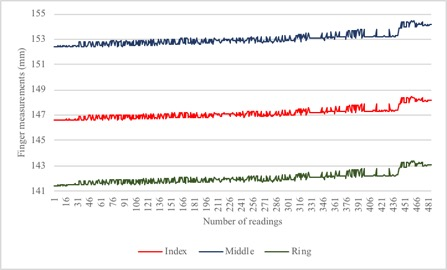
\includegraphics[width=1.0\textwidth]{Chapter4/Figs/FiveSecondScanGraph.jpg}
    \caption[Five Second hand scan graph]{Five Second hand scan graph}
    \label{fig:Five Second hand scan graph}
    \end{figure}
    
The significance of this data is prevalent when taking into consideration the distribution throughout the scan. It is of utmost importance to conistently extract concise data readings throughout the length of the scan. Thus, the standard deviation of the raw data correlating to the plotted data was calculated in an attempt to demonstrate the accuracy that the LMC provides (see Table ~\ref{table: Randomly selected data from five second scan}).

It is interesting to note that the longer the scan has progressed, the more varied the readings become. This is attributed to the instability that is associated with an unsupported hand being held in mid-air for any given period of time.

\section{Comparitive vector tolerance}

Despite the abovementioned LMC accuracy, the system shows slight deviation from one scan to the next. To provide an explicit limit regarding the deviation of the readings during a scan, it was decided to measure a tolerance range.

The manner within which this tolerance range was calculated involves comparing test data from user enrolment scan to that of the associated authentication scan. This data includes all of the users and their transformed vector combinations. With this data, the maximum tolerance range was extrapolated based on the variations produced by the system. As seen in Figure ~\ref{fig:Comparative vector tolerance} below, it was concluded that the maximum tolerance range for this data set is 5mm.

% Figure - Comparative vector tolerance
    
    \begin{figure}[htbp!] 
    \centering    
    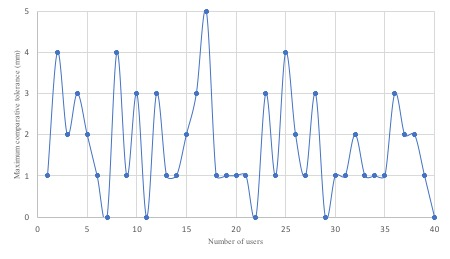
\includegraphics[width=1.0\textwidth]{Chapter4/Figs/ComparitiveVectorTolerance.jpg}
    \caption[Comparative vector tolerance]{Comparative vector tolerance}
    \label{fig:Comparative vector tolerance}
    \end{figure}

Upon further evaluation, with the tolerance range at a maximum of 5mm, the acceptance rates exponentially improved. This, however, increased the processing time to find a positive match within the tolerance range of the transformed vector. 

% Algorithm - check vector hash combinations

\begin{algorithm}
     \SetKwInOut{Input}{Input}
     \SetKwInOut{Output}{Output}
     
     \underline{function VectorCombinationsCheck} ( $transformedVector$, $count$)\;
     \Input{$transformedVector$}
     \Output{$result$}
     
      \tcp{transformedVector, low and high are \textbf{arrays}}
      $low$;
      $high$;
     
     $increment$ = 0;
     
     \If{$count$ = $transformedVector$.Length}{
        \textbf{return}\;
     }
     
     \For{($value$ in $transformedVector$)}{
        $increment$++\;
        
        \textbf{Array}.Copy($transformedVector$, $low$)\;
        $low$[count] = $transformedVector$[count] - $increment$\;
        \textbf{checkLowMatch} = GenerateHash($low$)\;
        \textbf{Array}.Copy($transformedVector$, $high$)\;
        $high$[count] = $transformedVector$[count] + $increment$\;
        \textbf{checkHighMatch} = GenerateHash($high$);
        \tcp{Recurse}
        \textbf{VectorCombinationsCheck}($low$, count + 1)\;
        \textbf{VectorCombinationsCheck}($high$, count + 1)\;
        
     }
     
     return $result$ = \textbf{VectorCombinationsCheck($transformedVector$)}
     
     
     \caption{Recursive algorithm to find possible vector combinations}
\end{algorithm}


\section{Overall system evaluation}

As deduced from Figure ~\ref{fig:System tolerance vs acceptance rates}, a zero-tolerance rate resulted in only a 12.5\% true acceptance rate. If this tolerance is then increased, the true acceptance rate also increases (e.g. 97.5\% with a 4mm tolerance) until a 100\% true acceptance rate is obtained at 5mm tolerance. 
When considering implementing this particular system approach, one needs to determine what risk factor is suitable within the authentication scenario. If the users that need to be authenticated are to be granted access to sensitive data/areas, then the tolerance range should be adjusted accordingly. The acceptance rate is drastically affected when using the maximum tolerance range. With such a high tolerance range, the false acceptance rate is also dramatically increased, but because of the two-factor authentication provided with the allocated PIN, the users are authenticated correctly.

% Figure - System tolerance vs acceptance rates
    
    \begin{figure}[htbp!] 
    \centering    
    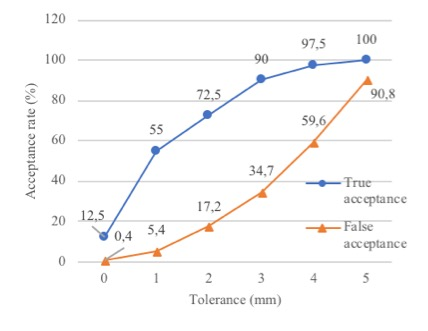
\includegraphics[width=1.0\textwidth]{Chapter4/Figs/ToleranceVsAcceptanceGraph.jpg}
    \caption[System tolerance vs acceptance rates]{System tolerance vs acceptance rates}
    \label{fig:System tolerance vs acceptance rates}
    \end{figure}


\section{Discussion}

The proposed technique has revealed several promising advantages by using a combination of the techniques specified in Section II. The LMC was found to be a stable and efficient hand geometry scanner. Also, the steganography techniques used in this paper were relatively easy to implement for use in this particular instance. By using PINs (to implement two-factor authentication) the security is enhanced and aids in achieving cancelability for storing biometrics. The proposed framework ensured that the system provided results that were reliable and efficiently obtained.
Bearing in mind the abovementioned advantages, one must acknowledge some disadvantages are present when using this approach. This system was only exposed to limited testing and the authentication accuracy and robustness will need to be measured using a formal evaluation. In order to fully explore the system’s functionality, one would have to extensively test the use of this framework on a larger scale. This will form part of the ongoing research.


\section{Data}

\subsection{Extraction}

\subsection{Analysis}

% \section{Optimisation}

\section{Algorithm evaluation}

\section{Conclusion}

\section{Chapter summary}